\documentclass[a4paper]{article}

\usepackage[utf8]{inputenc}
\usepackage[T1]{fontenc}
\usepackage{graphicx}
\usepackage[frenchb]{babel}
\usepackage{amsmath}
\usepackage{listings}

% define our color
\usepackage{xcolor}

% code color
\definecolor{ligthyellow}{RGB}{250,247,220}
\definecolor{darkblue}{RGB}{5,10,85}
\definecolor{ligthblue}{RGB}{1,147,128}
\definecolor{darkgreen}{RGB}{8,120,51}
\definecolor{darkred}{RGB}{160,0,0}

% other color
\definecolor{ivi}{RGB}{141,107,185}


\lstset{
    language=scilab,
    captionpos=b,
    extendedchars=true,
    frame=lines,
    numbers=left,
    numberstyle=\tiny,
    numbersep=5pt,
    keepspaces=true,
    breaklines=true,
    showspaces=false,
    showstringspaces=false,
    breakatwhitespace=false,
    stepnumber=1,
    showtabs=false,
    tabsize=3,
    basicstyle=\small\ttfamily,
    backgroundcolor=\color{ligthyellow},
    keywordstyle=\color{ligthblue},
    morekeywords={include, printf, uchar},
    identifierstyle=\color{darkblue},
    commentstyle=\color{darkgreen},
    stringstyle=\color{darkred},
}

\begin{document}

\title{VISA -- TP3 : stéréovision dense}
\author{Arnaud Cojez}
\date{mardi 4 octobre 2016}

\maketitle

\newpage
\tableofcontents
\newpage
%----------------------------------------------------------------------------------------
%	INTRODUCTION
%----------------------------------------------------------------------------------------

\section{Introduction}

\subsection{Motivation}
Lors du dernier TP sur la mise en correspondance stéréoscopique, nous avons utilisé une méthode de stéréoscopie dite "éparse". Celle-ci consistait en l'utilisation d'une sélection de points pour la mise en correspondance entre 2 images. Ce qui nous permettait de retrouver des informations de profondeur grâce à 2 projections de la même scène, avec des points de vues différents.\\

Nous allons ici mettre en œuvre une méthode de mise en correspondance stéréoscopique dense. C'est-à-dire que nous allons utiliser tous les pixels d'une projection, et non une sélection de points, afin de calculer la disparité entre l'image gauche et l'image droite.

\subsection{La stéréovision dense}

Le but de cette méthode est de créer une carte de disparité entre chaque pixel de deux projections. La disparité correspond à la différence d'abscisse entre deux points considérés comme homologues pour les deux images.\\

Pour simplifier les calculs, nous allons utiliser une configuration de stéréoscope canonique. C'est une configuration dans laquelle :
\begin{itemize}
\item les deux caméras sont identiques ;
\item les axes optiques sont parallèles ;
\item les deux capteurs d’image sont coplanaires ;
\item les lignes horizontales des capteurs sont confondues.\\
\end{itemize}

Cette configuration possède plusieurs avantage qui nous soulagent de certaines étapes d'estimations ou de réctifications (ex. réctification épipolaire). C'est pour cette raison que nous allons utiliser une méthode de stéréovision dense, avec des images issues d'un stéréoscope canonique.\\

Nous allons utiliser cette méthode sur ces deux images en niveau de gris.
\begin{figure}[h]
\begin{center}
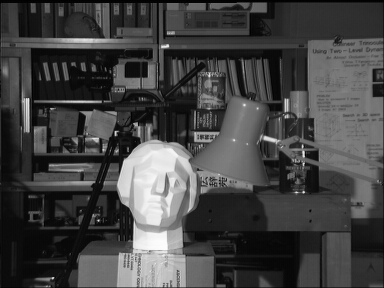
\includegraphics[width=170px]{left.png}
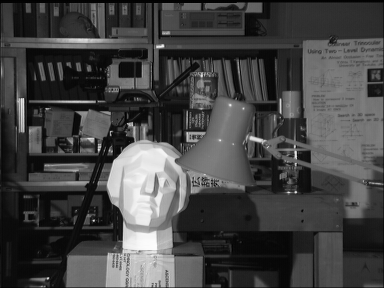
\includegraphics[width=170px]{right.png}
\end{center}
\caption{Image gauche et Image droite}
\end{figure}

\clearpage
%----------------------------------------------------------------------------------------
%	SIMILARITÉ PAR SSD
%----------------------------------------------------------------------------------------

\section{Calcul de l'image de disparité gauche}

Pour calculer l'image de disparité relative aux points de l'image de gauche, nous devons suivre plusieurs étapes.

\subsection{Image intermédiaire minSSD}

Cette étape consiste à calculer l'image intermédiaire minSSD. Cette matrice est de la même taille que l'image de gauche donnée en paramètre.
Chaque élément de cette matrice se verra assigner la valeur $dMinSSD = (2 * iWindowHalfSize + 12 * iWindowHalfSize + 1)^2 * 512.0$, qui correspond au maximum possible de SSD (sum of squared differences).

\begin{lstlisting}
Mat iviLeftDisparityMap(const Mat& mLeftGray,
                        const Mat& mRightGray,
                        int iMaxDisparity,
                        int iWindowHalfSize) {
  [...]

  Mat mMinSSD(mLeftGray.size(), CV_64F);

  [...]

  // Initialisation de l'image du minimum de SSD
  dMinSSD = pow((double)(2 * iWindowHalfSize + 1), 2.0) * 512.0;
  for (iRow = iWindowHalfSize;
      iRow < mMinSSD.size().height - iWindowHalfSize;
      iRow++) {
      // Pointeur sur le debut de la ligne
      pdPtr1 = mMinSSD.ptr<double>(iRow);
      // Sauter la demi fenetre non utilisee
      pdPtr1 += iWindowHalfSize;
      // Remplir le reste de la ligne
      for (iCol = iWindowHalfSize;
          iCol < mMinSSD.size().width - iWindowHalfSize;
          iCol++)
              *pdPtr1++ = dMinSSD;
  }

  [...]

}
\end{lstlisting}

Nous avons donc les valeurs de SSD maximales dans cette matrice, valeurs que nous tenterons de réduire dans la partie suivante, en cherchant la SSD minimale pour chaque point.

\subsection{Image intermédiaire mSSD}

Maintenant que nous avons cette base des SSD maximum, nous pouvons calculer les vraies SSD, qui seront stockées temporairement dans la matrice mSSD.
Le but est de calculer la SSD minimale de chaque point en se servant des pixels de la même ligne. Le résultat obtenu sera stocké dans la matrice mSSD. Si le résultat est inférieur à la SSD minimale (contenue dans mMinSSD), alors celui-ci viendra y remplacer l'ancienne valeur.

La SSD est calculée dans iviComputeLeftSSDCost, méthode que nous implémenterons par la suite.

\begin{lstlisting}
Mat iviLeftDisparityMap(const Mat& mLeftGray,
                        const Mat& mRightGray,
                        int iMaxDisparity,
                        int iWindowHalfSize) {
  [...]

  Mat mSSD(mLeftGray.size(), CV_64F);

  [...]

    // Boucler pour tous les decalages possibles
    for (iShift = 0; iShift < iMaxDisparity; iShift++) {
        // Calculer le cout SSD pour ce decalage
        mSSD = iviComputeLeftSSDCost(mLeftGray, mRightGray,
                                     iShift, iWindowHalfSize);
        // Mettre a jour les valeurs minimales
        for (iRow = iWindowHalfSize;
            iRow < mMinSSD.size().height - iWindowHalfSize;
            iRow++) {
            // Pointeurs vers les debuts des lignes
            pdPtr1 = mMinSSD.ptr<double>(iRow);
            pdPtr2 = mSSD.ptr<double>(iRow);
            pucDisparity = mLeftDisparityMap.ptr<unsigned char>(iRow);
            // Sauter la demi fenetre non utilisee
            pdPtr1 += iWindowHalfSize;
            pdPtr2 += iWindowHalfSize;
            pucDisparity += iWindowHalfSize;
            // Comparer sur le reste de la ligne
            for (iCol = iWindowHalfSize;
                iCol < mMinSSD.size().width - iWindowHalfSize;
                iCol++) {
                // SSD plus faible que le minimum precedent
                if (*pdPtr1 > *pdPtr2) {
                    *pucDisparity = (unsigned char)iShift;
                    *pdPtr1 = *pdPtr2;
                }
                // Pixels suivants
                pdPtr1++; pdPtr2++; pucDisparity++;
            }
        }
    }

  [...]

}
\end{lstlisting}

\subsection{Calcul de la SSD pour l'image gauche}

\begin{equation}
\sum_{i=-w_x}^{w_x} \sum_{i=-w_y}^{w_y} (I_l(x_l+i,y+j)-I_r(x_l+1-s,y+j))^2
\end{equation}

\begin{lstlisting}
  
\end{lstlisting}
\clearpage
%----------------------------------------------------------------------------------------

%----------------------------------------------------------------------------------------
%	CONCLUSION
%----------------------------------------------------------------------------------------

\section{Conclusion}

\clearpage
%----------------------------------------------------------------------------------------

\section{Annexe}

\end{document}
